\section{Set definitions for the RMPC}
\label{sec:set definitions}

Algorithm \ref{alg:RMPC} and the problem $\Pk{k}$ \eqref{eq:nom mpc} use a number of constraint sets to ensure recursive feasibility of the successive RMPC optimizations, namely: 
inner approximations of the admissible input sets $\ua{V}_{k+j|k}$, 
bounding sets for the ($T$-mapped) estimation error $\tE_{k+j|k}$, 
bounding sets for the process noise $\What_{k+j|k}$, 
and the largest error and noise sets $\tE_{max}$ and $\What_{max}$.
In this section we show how these sets are defined and computed.

 \subsection{Approximating the reach set of the nonlinear system}
 \label{sec:x reach}

 First we show how to compute an outer-approximation of the $j$-step reach set of the nonlinear system, starting at time $k$, $ \oaXset{k+j}{k}$.
This is needed for computing $\ua{V}_{k+j|k}$ and $\tE_{k+j|k}$.
 
 In all but the simplest systems, forward reachable sets cannot be computed exactly.
 To approximate them we may use a reachability tool for nonlinear systems like RTreach \cite{JohnsonBCS16_Rtreach}.
 A reachability tool computes an outer-approximation of the reachable set of a system starting from some set $\Xc \subset X$, subject to inputs from a set $U$, for a duration $T \geq 0$. 
 Denote this approximation by $\RT{\Xc}$, so $x(T) \in \RT{\Xc}$ for all $T$, $x(0) \in \Xc$ and $u:[0,T] \rightarrow U$.
 
 At time $k$, the state estimate $\hx_{k}$ is known.
 Therefore $x_k = \hx_{k} - e_k \in \hx_{k} \oplus (-E) \defeq \Xset{k}{k}$.
 Propagating $\Xset{k}{k}$ forward one step through the continuous-time nonlinear dynamics yields $\Xset{k+1}{k}$, which is outer-approximated by $\RT{\Xset{k}{k}}$.
 The state estimate that the system will receive at time $k+1$ is therefore bound to be in the set $\RT{\Xset{k}{k}}  \oplus E$.
 Since $0 \in E$, we maintain $\Xset{k+1}{k} \subset \RT{\Xset{k}{k}}  \oplus E$.
 We define the outer-approximate reach set at $k+1$, computed at time $k$, to be 
 \begin{equation*}
 \label{eq:def Xk}
 \oaXset{k+1}{k} \defeq  \RT{\Xset{k}{k}}  \oplus E \oplus  (-E)
 \end{equation*}
 (The reason for adding the extra $-E$ term will be apparent in the proof to Thm. \ref{th:robust_feas}).

 More generally, for $1 \leq j \leq N$, we define the $j$-step approximation computed at time $k$ to be
 \begin{eqnarray}
 \label{eq:def Xkj}
 \oaXset{k}{k} &\defeq&   \hx_{k} \oplus (-E) 
 \nonumber
 \\
 \oaXset{k+j}{k} & \defeq& \RT{\oaXset{k+j-1}{k}} \oplus E \oplus (-E) 
 \end{eqnarray}
  Fig. \ref{fig:overreach_NL} shows a visualization of this approach.
 The following holds by construction:
 \begin{lemma}
 	\label{lemma:xreach}
 	For any time $k$ and step $j \geq 1$,
 	$\Xset{k+j}{k} \subset \oaXset{k+j}{k}$.
 \end{lemma}
 
 
 \begin{figure*}
 	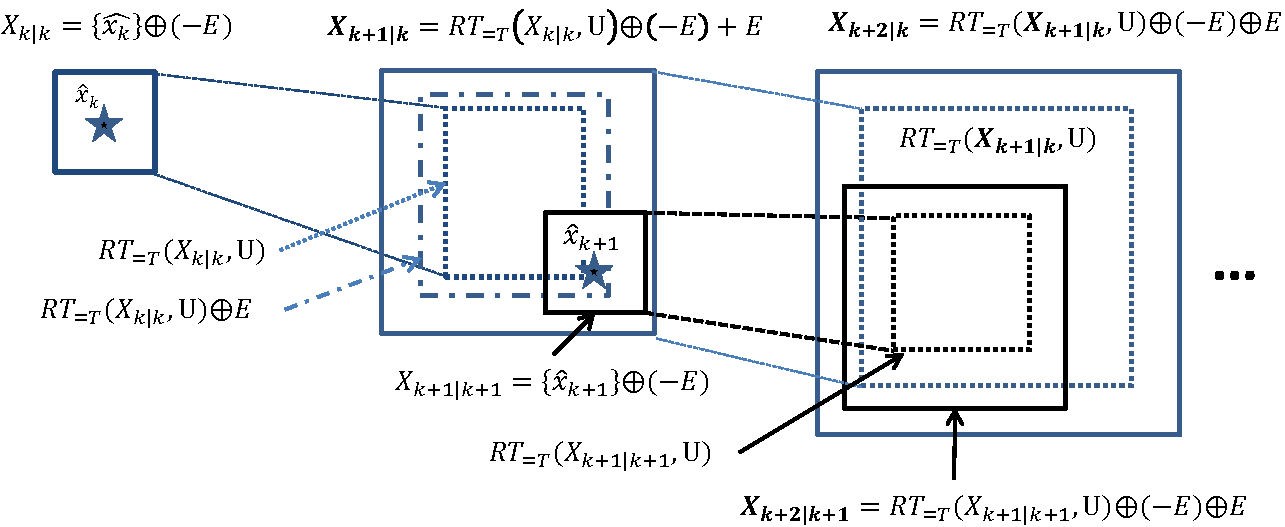
\includegraphics[scale=0.75]{figs/OverReachFigure_NL_scissored.pdf}
 	\caption{The outer-approximated reach sets for $x_{k+j}$, computed at time steps $k,k+1$, used to compute $\tE_{k+j|k}$, $\ua{V}_{k+j|k}$. }
 	\label{fig:overreach_NL}
 \end{figure*}
 
 This construction of $\oaXset{k+j}{k}$ permits us to prove recursive feasibility of the RMPC controller, because it causes the constraints of the RMPC problem setup at time $k+1$ to be consistent with the constraints of the RMPC problem setup at time $k$.

\subsection{Approximating the bounding sets for the input}
\label{sec:approx input sets}
Given $x \in X$, define the set $V(x) \defeq \{v \in \Re^{\dimV} \such u(x) = R^{-1}(x)[b(x)+v] \in U\}$.
We assume that there exist functions $\ua{v}_i, \oa{v}_i: X \rightarrow \Re$ s.t. for any $x$, $V(x) = \{[v_1,\ldots,v_{\dimV}]^T \such \ua{v}_i(x;U) \leq v_i \leq \oa{v_i}(x;U) \}$.
Because in general $V(x)$ is not a rectangle, we work with inner and outer rectangular approximations of $V(x)$.
Specifically, let $\Xc$ be a subset of $X$.
Define the inner and outer bounding rectangles, respectively
\[\ua{V}(\Xc) \defeq \{[v_1,\ldots,v_{\dimV}]^T \such \max_{x\in \Xc} \ua{v}_i(x;U)  \leq v_i \leq \min_{x \in \Xc} \oa{v}_i(x;U) \} \]
\[\oa{V}(\Xc) \defeq \{[v_1,\ldots,v_{\dimV}]^T \such \min_{x\in \Xc} \ua{v}_i(x;U)  \leq v_i \leq \max_{x \in \Xc} \oa{v}_i(x;U) \} \]

By construction, we have for any subset $\Xc \subset X$
\begin{equation}
\label{eq:Vbounds}
\ua{V}(\Xc) \subseteq \cap_{x \in \Xc} V(x) \subset \oa{V}(\Xc)
\end{equation}
If two subsets of $X$ satisfy $\Xc_1 \subset \Xc_2$, then it holds that 
\begin{equation}
\label{eq:V inclusions}
\ua{V}(\Xc_2) \subset \ua{V}(\Xc_1), \; \oa{V}(\Xc_1) \subset \oa{V}(\Xc_2)
\end{equation}

We can compute:
\begin{equation}
\label{eq:Vkj Vmax}
\ua{V}_{k+j|k}  = \ua{V}(\oa{X}_{k+j|k}), \; \ua{V}_{inner-global} = \ua{V}(X)
\end{equation}
In practice we use interval arithmetic to compute these sets since $\oaXset{k+j}{k}$ and $U$ are hyper-intervals.
Fig. \ref{fig:err bounds toy} shows these sets for the running example.
\begin{figure}
	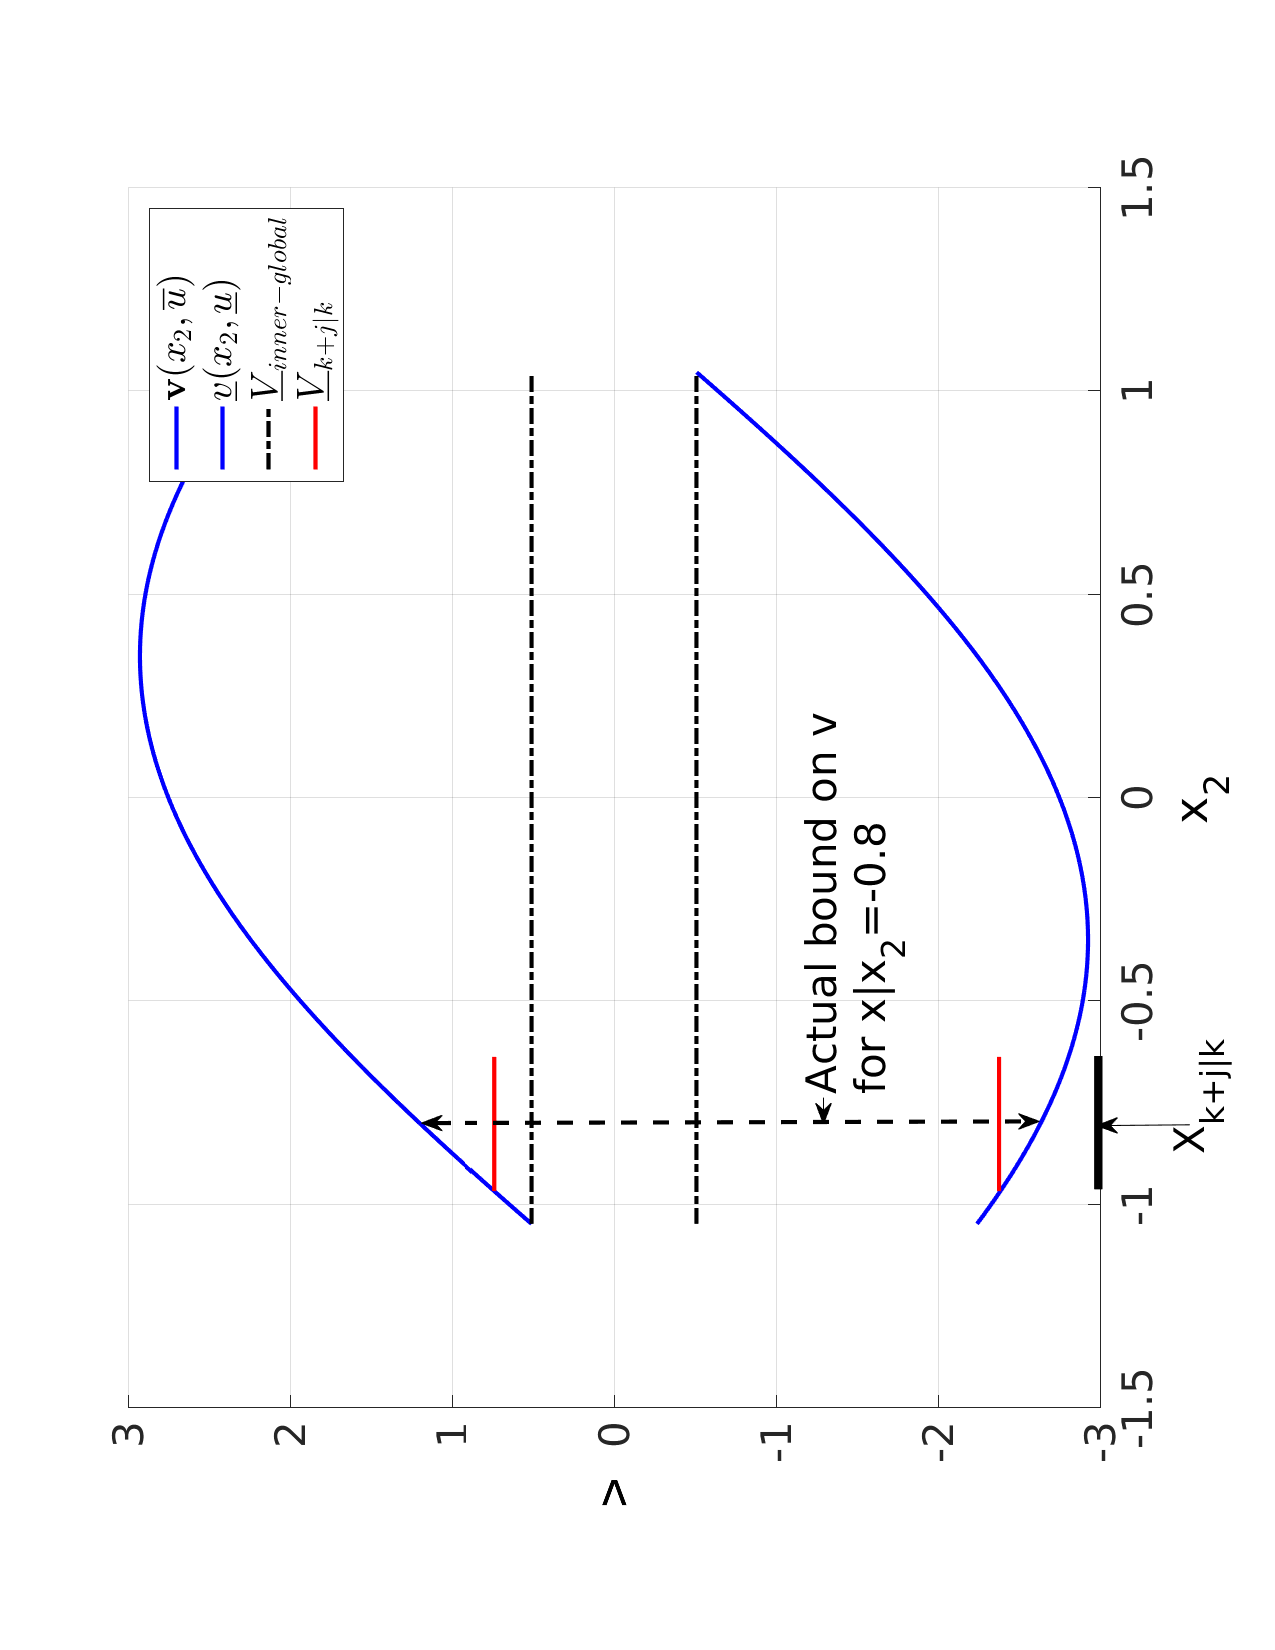
\includegraphics[angle=270,width=0.49\textwidth]{figs/InputToy.pdf}
	\caption{Local and global inner approximations of input constraints for running example, with $\oa{X}_{k+j|k} =  [-\pi/4,0]\times[-0.9666,-0.6283]$ for some $k,j$ and $U = [-2.75,2.75]$. Color in online version.}
	\label{fig:err bounds toy}
\end{figure}


\subsection{Approximating the bounding sets for the disturbances}
\label{sec:approx dist}
We will also need to define containing sets for the state estimation error in $z$ space:
recall that $\hat{z}_k = T(\hat{x}_k) = T(x_k+e_k)$. 
%******************
We use a Taylor expansion
\begin{eqnarray}
\label{eq:taylor expansion T}
\hat{z}_k &=& T(x_k) + \underbrace{\frac{dT}{dx}(x_k)}_{M(x_k)}e_k+ \underbrace{\frac{1}{2}e_k^T \frac{d^2T}{dx^2}(c)e_k}_{r_k(c)}, c \in x_k + E \nonumber 
\\
&=& T(x_k) + M(x_k)e_k+ r_k(c), c \in x_k + E \nonumber
\\
&=& T(x_k) + h_{k}+ r_k(c), c \in x_k + E \nonumber
\end{eqnarray}

The remainder term $r_k(c)$ is bounded in the set $\cup_{c \in \{x_k\} \oplus  E}   \frac{1}{2}e^T\frac{d^2T}{dx^2}(c)e$.
Thus when setting up $\Pk{k}$, at the $j^{th}$ step, 
$r_{k+j|k} \in D_{k+j|k} \defeq \cup_{c \in \oaXset{k+j}{k} \oplus  E}   \frac{1}{2}e^T\frac{d^2T}{dx^2}(c)e $,
where $\oa{X}_{k+j|k}$ is the reach set computed in \eqref{eq:def Xkj}.

The error $h_{k}$ lives in 
$\cup_{x\in X_{k}, e \in E}M(x)e$.
Thus when setting up $\Pk{k}$, the error $h_{k+j|k}$ lives in $\cup_{x \in \oa{X}_{k+j|k}}M(x)E$.
Finally the rectangular over-approximation of this set is 
\begin{eqnarray}
\label{eq:H}
H_{k+j|k} = \{h \such \sum_{\ell=1}^{\dimX} \min_{x \in \oa{X}_{k+j|k}, e \in E} M_{i\ell}(x)e(\ell)  \leq h(i) 
\nonumber 
\\
\leq \sum_{\ell=1}^{\dimX} \max_{x \in \oa{X}_{k+j|k}, e \in E} M_{i\ell}(x)e(\ell) \}
\end{eqnarray}
where $M_{i\ell}$ is the $(i,\ell)^{th}$ element of matrix $M$ and $h(\ell)$ is the $\ell^{th}$ element of $h$.

Therefore the state estimation error $h_{k+j|k} + r_{k+j|k}$ is bounded in the set $H_{k+j|k} \oplus D_{k+j|k}$. 
In the experiments we ignore the remainder term $D_{k+j|k}$ based on the observation that $e_k$ is small relative to the state $x_k$. Thus we use:
\begin{eqnarray}
\label{eq:tildeE}
\tE_{k+j|k} = H_{j+k|j}
\end{eqnarray}

\begin{exmp}
For the running example \eqref{eq:toy_dynamics}, we have $M = [1 ,  0;0 ,\cos(x_2)]$. 
If the estimation error $e$ (in radians) is bounded in $E = \lbrace e| ||e||_{\infty} \leq 0.0227\rbrace$,
then the relative linearization error, averaged over several realizations of the error, is less than $2\cdot 10^{-3}$.
\exmend
\end{exmp}

We also need to calculate containing sets for the process noise $\hw$.
Recall that for all $k,j$, 
$\hz_{k+j+1} =  A\hz_{k+j} + Bv_k + \hw_{k+j+1}$.
Therefore 
\begin{equation}
\label{eq:What}
\hw_{k+j+1} \in \What_{k+j+1|k} \defeq W \oplus \tE_{k+j+1|k} \oplus(-A\tE_{k+j|k})
\end{equation}

We also define the set $\tE_{max}$, which is necessary for the terminal constraints of Eq. \eqref{eq:P_f_def}. $\tilde{E}_{max}$ represents the worst case bound on the estimation error $\te_{k}$, and is computed similar to Eq. \eqref{eq:tildeE}, but over the entire set $X$. %and not reachable subsets of it:

\begin{equation}
\label{eq:EtildeMax}
\sum_{\ell=1}^{n} \min_{x \in X, e \in E} M_{i\ell}(x)e(\ell)  \leq \te_{k}(i)  \leq \sum_{\ell=1}^{n} \max_{x \in X, e \in E} M_{i\ell}(x)e(\ell)
\end{equation}

$\What_{max}$ is then defined as:
\begin{equation}
\What_{max} = W \oplus \tilde{E}_{max} \oplus (-A\tilde{E}_{max})
\end{equation}

For the running example, Fig. \ref{fig:err_bound_toy} shows the set $\tE_{max}$ and $\tilde{E}_{k+j|k}$ computed by Eqs. \eqref{eq:tildeE} and \eqref{eq:EtildeMax}. for an arbitrary  $\oa{X}_{k+j|k} =  [-\pi/4,0]\times[-0.9666,-0.6283]$. It also shows 1000 randomly generated values for $T(\hat{x})-x$ (for randomly generated $e \in E$ and $x \in \oa{X}_{k+j|k}$), and all fall inside $\tilde{E}_{k+j|k}$.

%computed over $\Xc= [-\pi/4,0]\times[-0.9666,-0.6283]$. 
%This shows that considering a reach set $\chi \subseteq X$ to compute the error bound results in less conservatism than using the worst case error bound. It also shows randomised realizations of the error for randomly selected $x \in \chi$ and $e \in E$, which %are all contained in the bounding set $\tilde{E}_{\chi}$.

\begin{figure}
	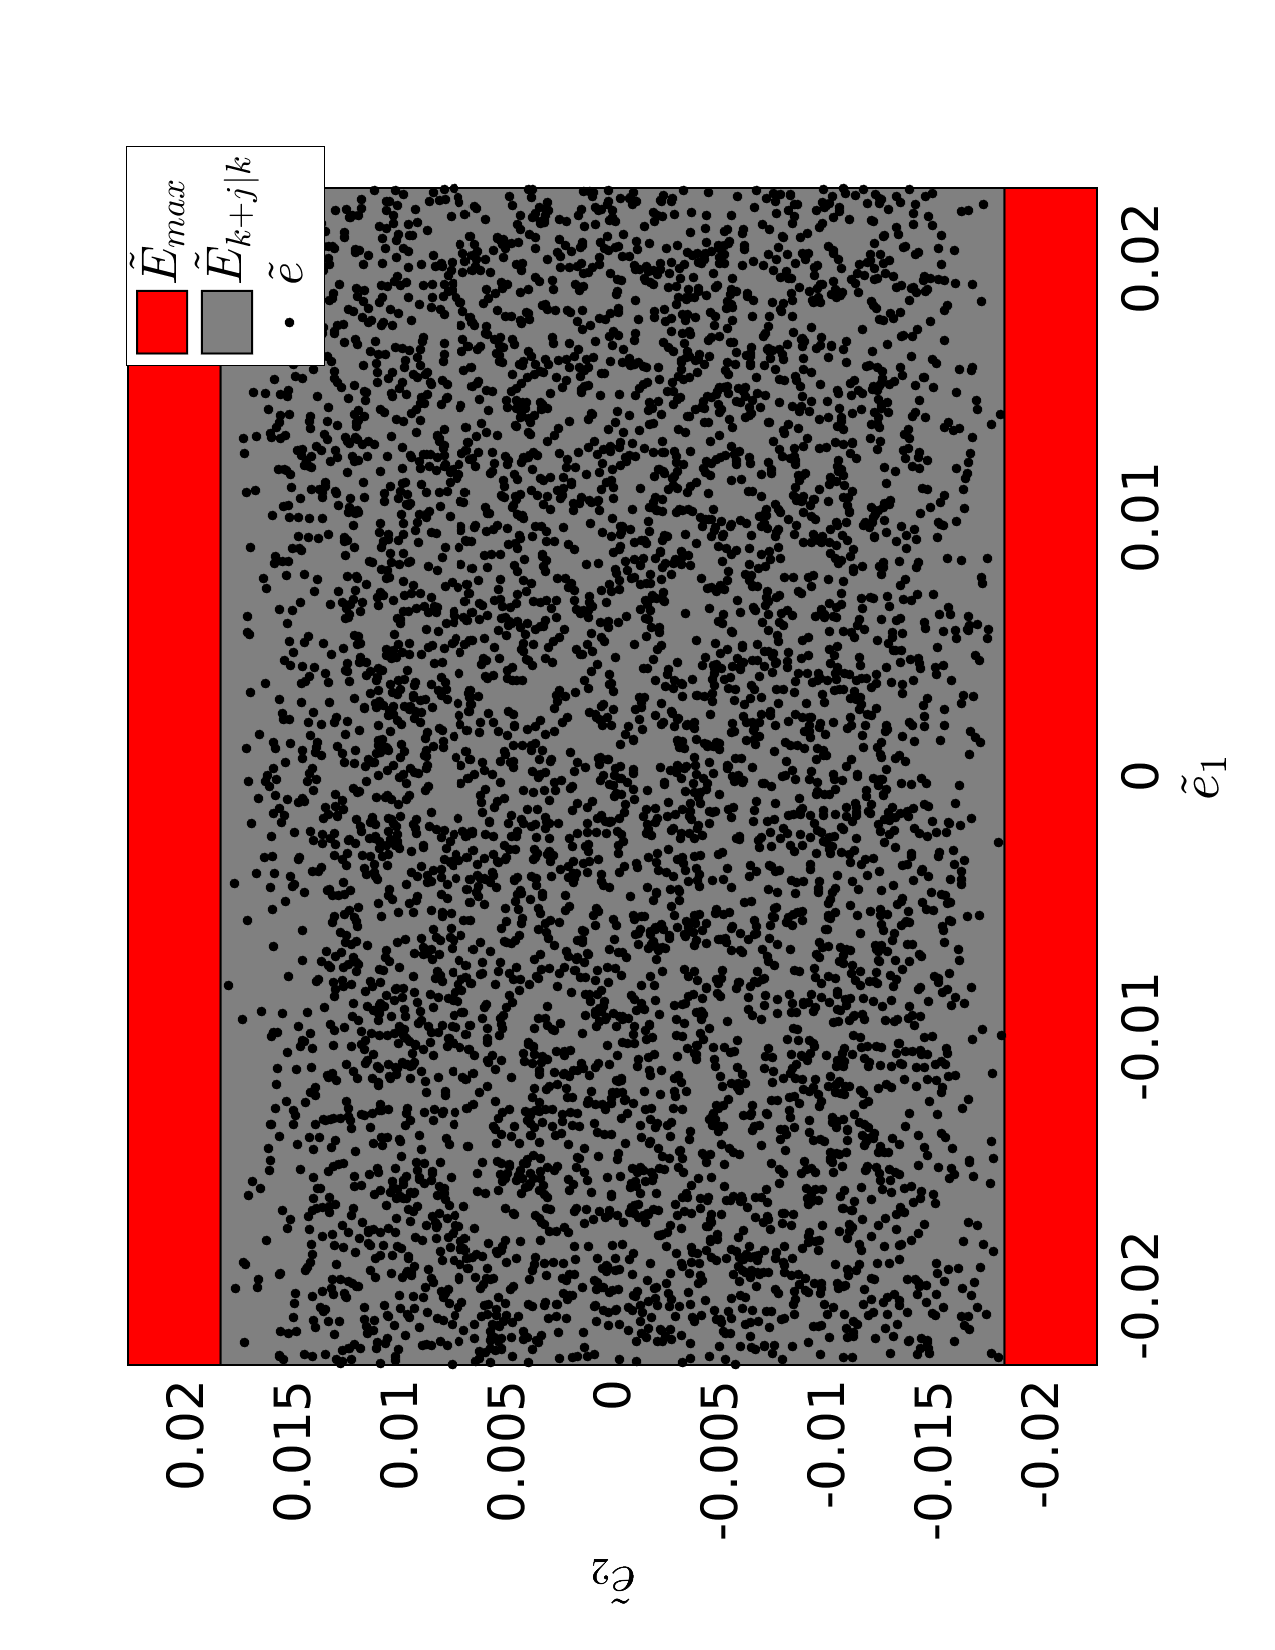
\includegraphics[angle=270,width=0.49\textwidth]{figs/Err_Bounds_toy.pdf}
	\caption{The error sets $\tilde{E}_{max}$ and $\tilde{E}$ computed over an arbitrary $\oa{X}_{k+j|k}$. Also shown are realizations of $\te \defeq T(\hx) - T(x)$ for randomly chosen $x \in \Xc$. Color in online version.}
	\label{fig:err_bound_toy}
\end{figure}


\subsection{Transforming between $x$-space and $z$-space}
\label{sec:transforming x to z}
Since we control the system in $z$-space, we need to compute a set $Z \subset \Re^{\dimZ}$ s.t. $z \in Z \implies x = \iT(z) \in X$, i.e. $Z \subset T(X)$.
Thus keeping the state $z$ of the linearized dynamics in $Z$ implies the nonlinear system's state $x$ remains in $X$.
Moreover, to check feasibility at time 0 of the MPC optimization, and for stability of the nonlinear dynamics, we need a subset $X_0 \subset X$ s.t. $x \in X_0 \implies z = T(x) \in Z$, i.e. $X_0 \subset \iT(Z)$.
Because $T$ can be an arbitrary diffeomorphism $Z$ and $X_0$ have to computed numerically.
\begin{enumerate}
	\item Let $Z_1 \subset \Re^{\dimZ}$ be the rectangle with bounds in the $i^{th}$ dimension $[ \min_{x \in X} T_i(x),  \max_{x \in X} T_i(x) ]$, $i=1,\ldots, \dimX$.
	This over-approximates $T(X)$. 
	Next we need to prune it so it under-approximates $T(X)$. 
	\item Define $z_{in} \defeq \min \{ \|z \|_0 \such z \in Z_1, \iT(z) \notin X\}$.
	$z_{in}$ is the smallest-norm inadmissible $z$ in $Z_1$.
	Thus all points in the $\ell_0$-ball of radius $\|z_{in}\|$,$B_z(0,\|z_{in}\|)$, are admissible, i.e. their pre-images via $\iT$ are in $X$.
	\item Let $R_z$ be the largest inscribed rectangle in $B_z(0,\|z_{in}\|)$.
	Now we need to get the $x$-set that maps to $R_z$  (or a subset of it).
	\item Let $X_1 \subset X$ be the rectangle with bounds in the $i^{th}$ dimension $[\min_{z \in R_{z}} \iT_i(z),  \max_{z \in R_{z}} \iT_i(z) ]$.
	Again, this is an over-approximation of $\iT(R_{z})$, so it needs to be pruned.
	\item Define $x_{in} = \inf \{\|x\|_0 \such x \in X_1, T(x) \notin R_{z}\}$.
	Then every point in the $\ell_0$-ball $B_x(0, \|x_{in}\|) \subset X$ maps via $T$ to $R_{z}$
\end{enumerate}
Therefore we choose $Z = R_z$ and $X_0$ to be the largest inscribed rectangle in $B_x(0,  \|x_{in}\|)$.

